\section{Project Requirement}

\noindent The project should implement ALU circuit described in \figref{fig:req_rtl}

\begin{figure}[!ht]
	\centering
	\caption{The RTL Diagram of the Required ALU}
	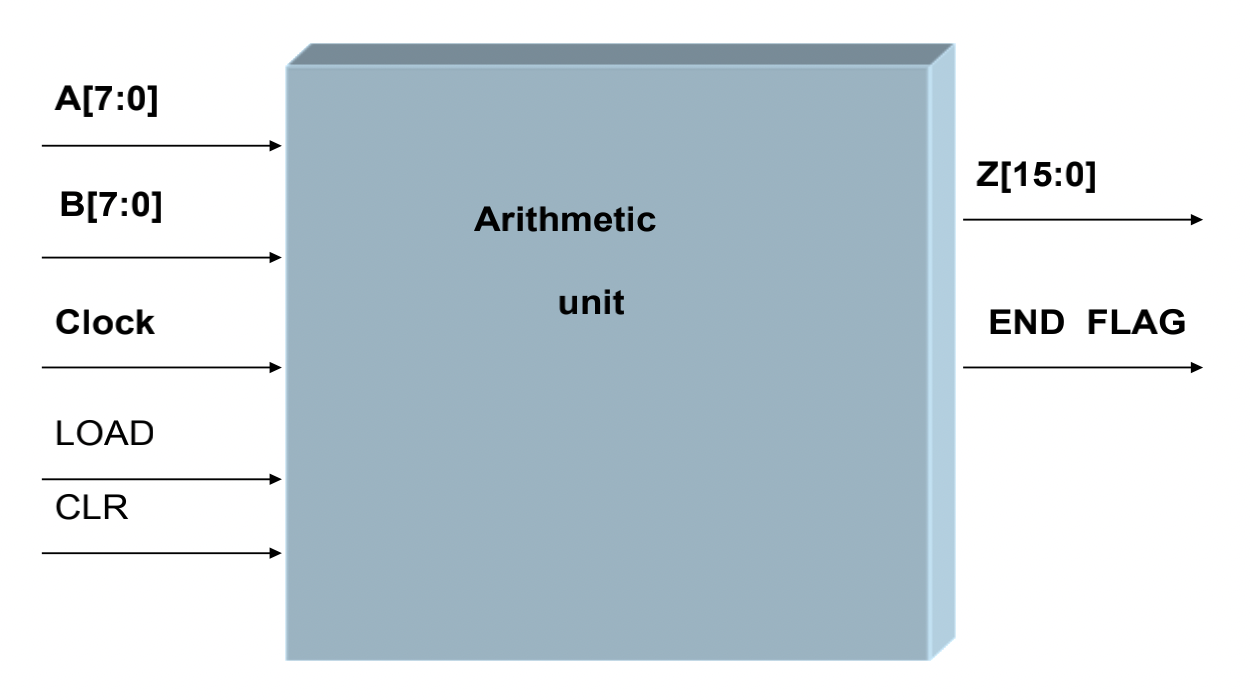
\includegraphics[width=0.5\textwidth]{../img/req_rtl.png}
	\label{fig:req_rtl}
\end{figure}

\noindent The project contains the following requirements for signals:

\begin{itemize}
	\item The operands \(A\) and \(B\) are latched into register RA and RB when \(LOAD\) signal transit from high to low.
	\item The unit outputs the results in 16-bit register RZ output port.
	\item Each calculation starts with a \(LOAD\) signal and ends with an \(END\_FLAG\) signal.
	\item The \(CLEAR\) signal will clear all registers to ‘0’.
	\item The unit performs the arithmetic operation until \(END\_FLAG\) becomes high.
	\item The 16-bit product shall be loaded into the 16-bit Z port.
	\item The design shall be structural.
\end{itemize}

\noindent The project contains the following extra features:

\begin{itemize}
	\item \textbf{(Accomplished)} Expansion of the method for 16 bits operand.
	\item \textbf{(Accomplished)} Pipelining of the design.
	\item Multiply Accumulate for additional operands.
\end{itemize}
